\chapter{Volar la búsqueda con ArduPilot}

\begin{enpocas}
Cómo se conectó ArduCopter a nuestra simulación: el modelo del dron para ArduPilot, sus parámetros, el nodo de misión, las ventanas, los comandos y la trayectoria en el mapa.
\end{enpocas}

\begin{lstlisting}[style=bash]
ros2 launch cuadrirotor_sim simulacion.launch.py vehiculo:=tarot650 mundo:=bosque_grande \
    controlador:=ardupilot mision:=busqueda
\end{lstlisting}

Con \cod{controlador:=ardupilot} el dron lo pilota ArduCopter 4.7.2 en lugar de los
controladores de ROS~2. Así se puede comparar el STA con un piloto automático real y
probar la misión con la misma interfaz (MAVLink) que tendría el dron físico.

\section{El vehículo para ArduPilot}
\label{sec:plugin-ap}

\cod{generar_modelo.py} genera también \cod{models/tarot650_ardupilot}: el mismo Tarot con
\begin{itemize}
  \item el plugin \cod{ArduPilotPlugin} (de \cod{ardupilot_gazebo}), que intercambia con el SITL el
        estado del dron y las salidas de los motores por UDP (puerto 9002, formato JSON, en
        \emph{lock-step}) y lee una IMU girada al marco NED;
  \item el sistema \cod{ComandosMotores} (\cod{cuadrirotor_gz_plugins}), que junta las cuatro salidas
        (un \cod{gz.msgs.Double} por motor, PWM de 1000--2000~µs escalado a 0--680~rad/s) en un solo
        \cod{gz.msgs.Actuators}, que es lo que espera \cod{MulticopterMotorModel}.
\end{itemize}
Así la física de los motores, el viento y el incendio son los mismos que con el PD y el STA.

\begin{lstlisting}[style=xml]
<plugin filename="ArduPilotPlugin" name="ArduPilotPlugin">
  <fdm_addr>127.0.0.1</fdm_addr>
  <fdm_port_in>9002</fdm_port_in>
  <lock_step>1</lock_step>
  <modelXYZToAirplaneXForwardZDown degrees="true">0 0 0 180 0 0</modelXYZToAirplaneXForwardZDown>
  <gazeboXYZToNED degrees="true">0 0 0 180 0 90</gazeboXYZToNED>
  <imuName>base_link::imu_sensor</imuName>
  <control channel="0">
    <jointName>rotor_0_joint</jointName>
    <type>COMMAND</type>
    <cmd_topic>/cuadrirotor/ap/motor_0</cmd_topic>
    <multiplier>680.0</multiplier>
    <servo_min>1000</servo_min>
    <servo_max>2000</servo_max>
  </control>
  <!-- ... canales 1 a 3 ... -->
</plugin>
<plugin filename="ComandosMotores" name="cuadrirotor::ComandosMotores">
  <entrada>/cuadrirotor/ap/motor_0</entrada>  <!-- ... motor_1 a motor_3 -->
  <salida>/cuadrirotor/command/motor_speed</salida>
</plugin>
\end{lstlisting}

\section{Parámetros de ArduCopter}

\cod{config/ardupilot/tarot650.parm} se carga sobre los del Iris de \cod{ardupilot_gazebo}:

\begin{lstlisting}
FRAME_CLASS     1        # quad
FRAME_TYPE      1        # X
MOT_PWM_MIN     1000
MOT_PWM_MAX     2000
MOT_THST_EXPO   1.0      # salida lineal en w, empuje en w^2: curva cuadrática pura
MOT_SPIN_ARM    0.08
MOT_SPIN_MIN    0.12
MOT_THST_HOVER  0.28     # (357/680)^2
MOT_HOVER_LEARN 2
ATC_RAT_RLL_P   0.08     # lazos de tasa más suaves que el Iris:
ATC_RAT_RLL_I   0.08     # empuje/peso ~3.6 y motores más lentos (30-50 ms)
ATC_RAT_RLL_D   0.002
ATC_RAT_PIT_P   0.08
ATC_RAT_PIT_I   0.08
ATC_RAT_PIT_D   0.002
ATC_RAT_YAW_P   0.2
ATC_RAT_YAW_I   0.02
\end{lstlisting}

\section{El nodo \texorpdfstring{\texttt{mision\_ardupilot}}{mision\_ardupilot}}

Corre con el Python de \cod{~/venv-ardupilot} (pymavlink) y se conecta a MAVProxy por
\cod{udp:127.0.0.1:14551}. Espera a que el EKF esté listo, pone el modo GUIDED, arma y despega con
\cod{MAV_CMD_NAV_TAKEOFF}. Después manda a 20~Hz \cod{SET_POSITION_TARGET_LOCAL_NED} con posición,
velocidad y guiñada:
\begin{itemize}
  \item con \cod{mision:=orbita} o \cod{hover}, la misma referencia que los controladores de ROS~2
        (\cod{dinamica.Referencia}); guarda el CSV con \cod{csv:=} en el formato de \cod{metricas.py};
  \item con \cod{mision:=busqueda}, despega a 5~m y después reenvía las consignas de
        \cod{busqueda_incendio}.
\end{itemize}
El paso de ENU a NED es $N = y$, $E = x$, $D = -z$ y $\psi_{NED} = \pi/2 - \psi$.

\begin{leccion}
Con el backend JSON, el marco local de ArduPilot (\cod{LOCAL_POSITION_NED}) \textbf{es} el mundo de
Gazebo, y el GPS de ArduPilot es el \emph{home} más la posición en Gazebo. La primera versión
restaba además el punto de salida $(-232,-232)$: todas las consignas llegaban corridas $\approx$330~m
al noreste. El dron patrullaba fuera de su ruta (de ahí unas detecciones de humo en rumbos
extraños) y en una corrida se estrelló contra un cerro (``\emph{Crash: Disarming}'').
Se encontró comparando el tlog de MAVProxy con la odometría de Gazebo. Ahora:
\begin{itemize}
  \item antes de armar se mide el desfase entre \cod{LOCAL_POSITION_NED} y la odometría (sale
        $\approx$(0.02, 0.01, 0.01)~m) y se descuenta, en lugar de suponerlo;
  \item el \emph{home} del SITL (\cod{-l}) es el origen del mundo (\cod{geo.ORIGEN}), así que el GPS
        de ArduPilot coincide con el del aviso del incendio.
\end{itemize}
\end{leccion}

\section{Las ventanas del SITL}
\label{sec:ventanas}

Con GUI se abren cinco ventanas, que \cod{ventanas_sitl.py} acomoda en columnas cuando aparecen
(con \cod{python-xlib}, por EWMH): la terminal \textbf{MAVProxy} arriba a la izquierda y al frente,
la consola y la terminal de ArduCopter debajo, Gazebo al centro y el mapa a la derecha.

\begin{figure}[H]
\centering
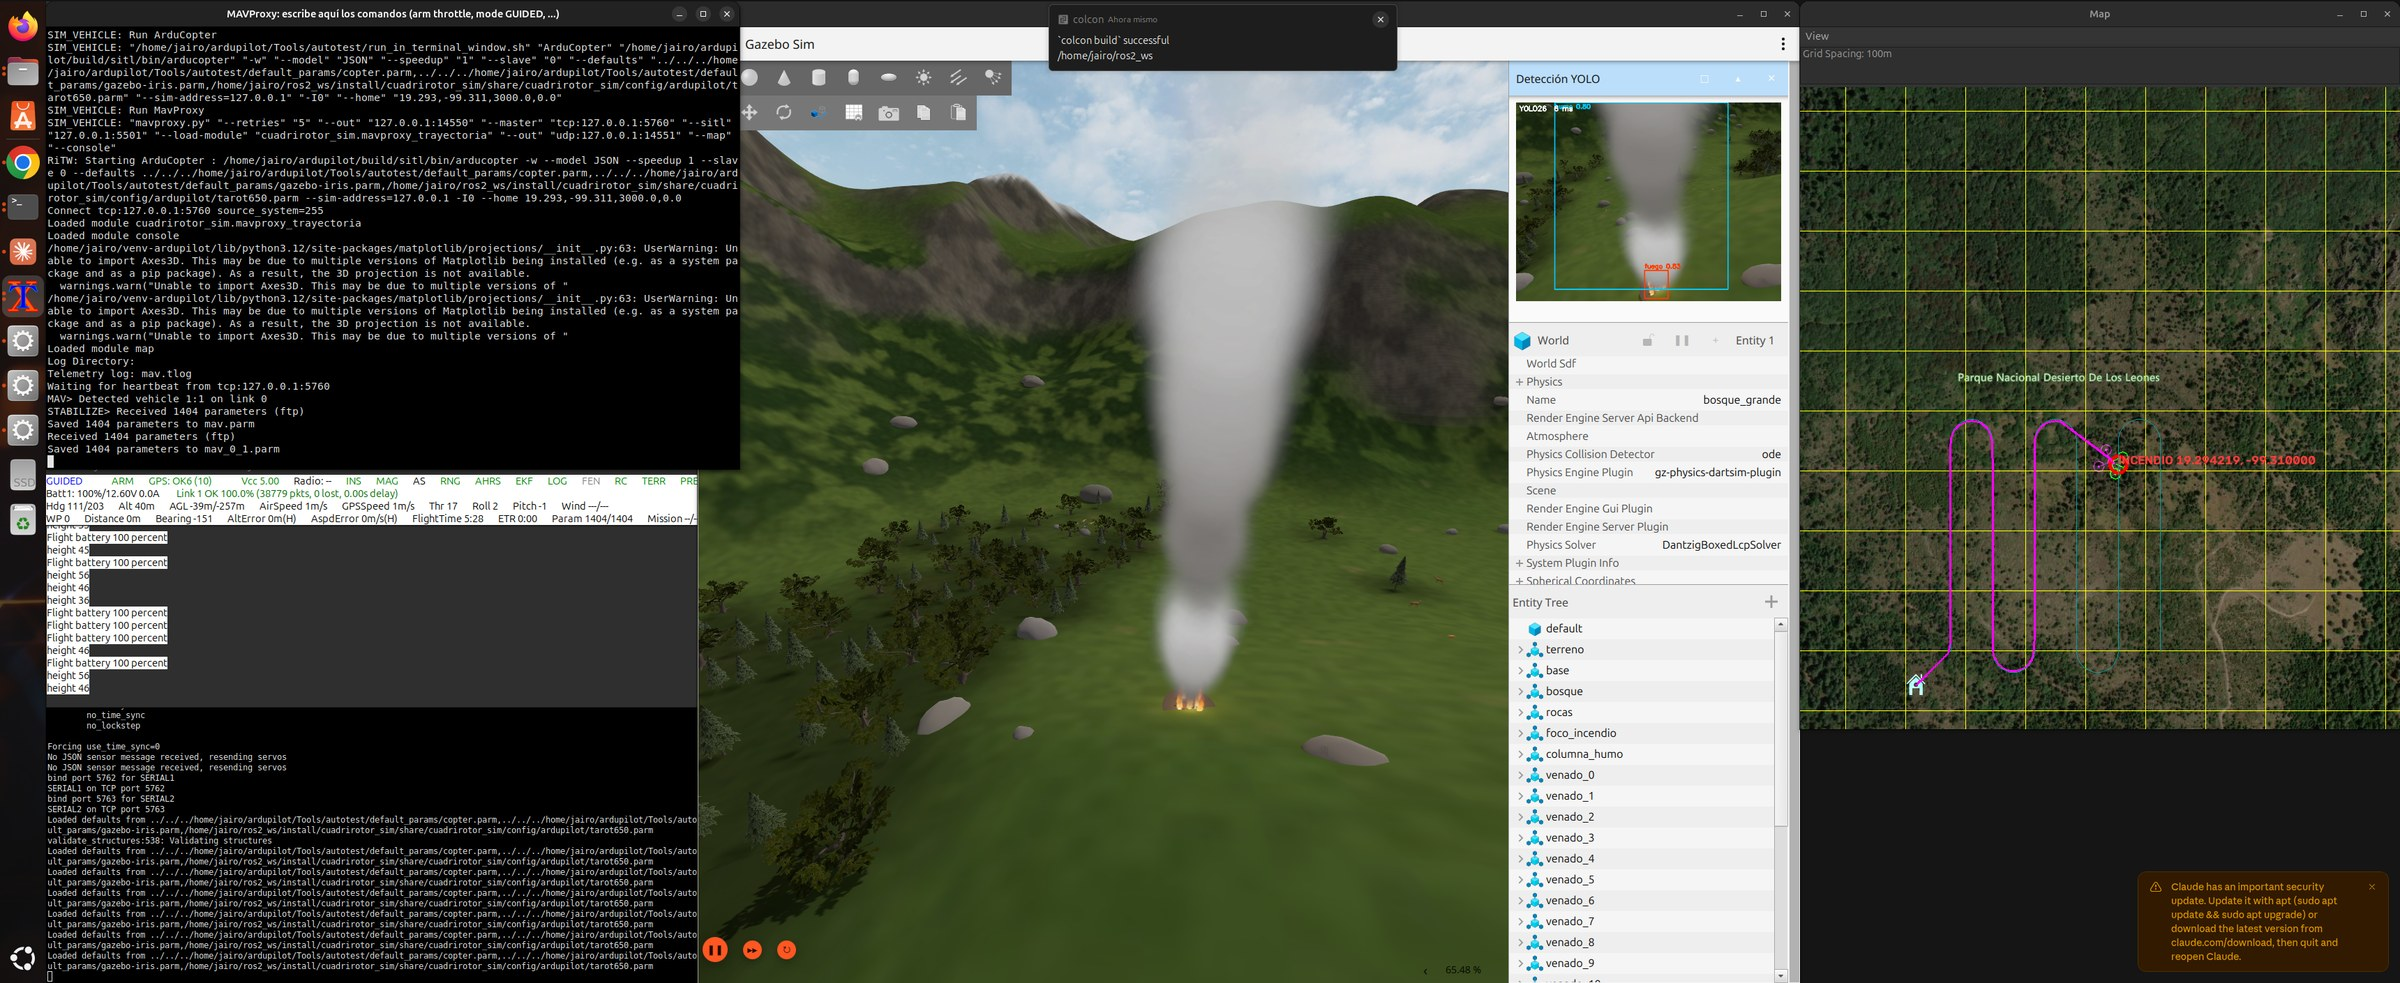
\includegraphics[width=\textwidth]{sitl_pantalla.jpg}
\caption{Pantalla durante la búsqueda con ArduPilot, al confirmarse el incendio.}
\end{figure}

\begin{description}
  \item[Terminal MAVProxy] sim\_vehicle.py corre dentro de ella: ahí queda el prompt de MAVProxy
        para escribir comandos.
  \item[Consola de MAVProxy] modo, armado, GPS, batería, altura y mensajes de ArduPilot.
  \item[Terminal ArduCopter] el proceso del SITL (antes se abría minimizada; ahora,
        \cod{SITL_RITW_TERMINAL} la abre a la vista).
  \item[Mapa] imagen satelital con el dron, el \emph{home} y lo que dibuja
        \cod{mavproxy_trayectoria}.
\end{description}

\begin{figure}[H]
\centering
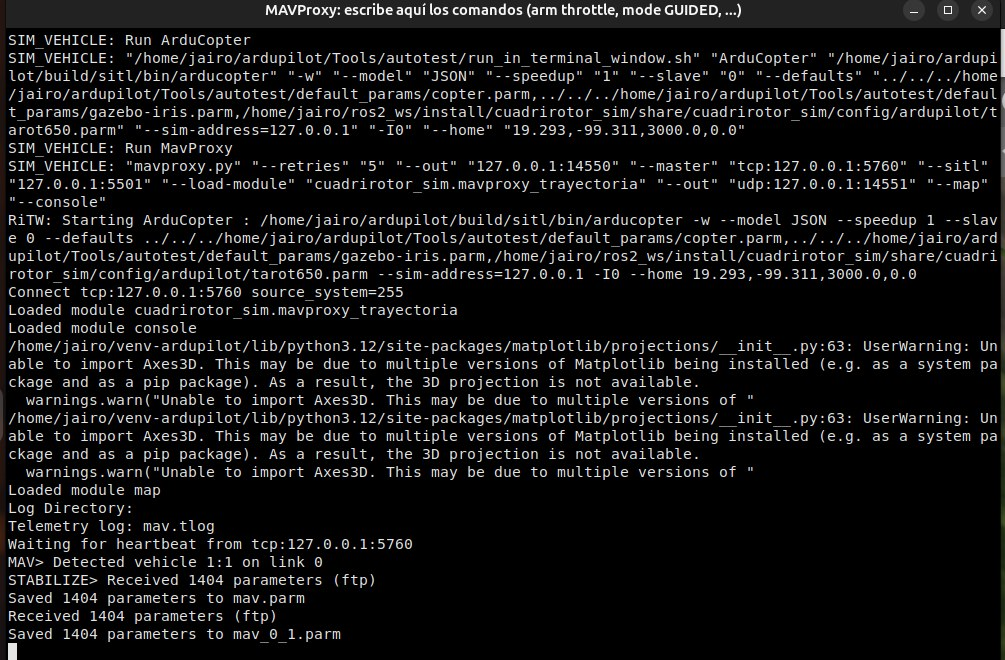
\includegraphics[width=0.56\textwidth]{sitl_mavproxy.jpg}\hfill
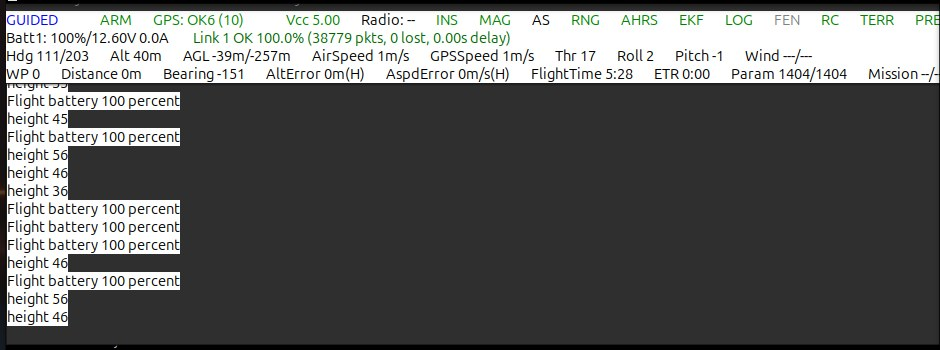
\includegraphics[width=0.42\textwidth]{sitl_consola.jpg}
\caption{Terminal de MAVProxy con su prompt (izquierda) y consola (derecha).}
\end{figure}

\subsection{Comandos útiles en el prompt de MAVProxy}

\begin{longtable}{>{\raggedright\arraybackslash}p{5cm}p{10cm}}
\toprule
\textbf{Comando} & \textbf{Efecto} \\ \midrule \endhead
\cod{mode GUIDED} & modo guiado (el que usa la misión) \\
\cod{arm throttle} & arma los motores \\
\cod{takeoff 10} & despega a 10~m (en GUIDED y armado) \\
\cod{mode LOITER} / \cod{mode BRAKE} & se queda en el lugar \\
\cod{mode RTL} & regresa a la base y aterriza \\
\cod{mode LAND} & aterriza donde está \\
\cod{disarm} & desarma (en tierra) \\
\cod{param show MOT_*} / \cod{param set NOMBRE valor} & ver y cambiar parámetros \\
\cod{trayectoria borrar} / \cod{ocultar} / \cod{mostrar} & controla el dibujo de la trayectoria en el mapa \\
\bottomrule
\end{longtable}

\begin{aviso}
Si se toma el control desde MAVProxy (por ejemplo \cod{mode RTL}), \cod{mision_ardupilot} sigue
enviando consignas, que solo surten efecto en GUIDED: al volver a \cod{mode GUIDED} el dron retoma
la búsqueda.
\end{aviso}

\section{La trayectoria en el mapa}

El módulo de MAVProxy \cod{cuadrirotor_sim.mavproxy_trayectoria} (se carga con
\cod{--load-module} cuando hay GUI) dibuja:
\begin{itemize}
  \item en magenta, \textbf{toda} la trayectoria recorrida (un punto cada 2~m de la posición GPS),
        en lugar de la estela de 12~s que trae MAVProxy;
  \item en cian, la ruta planeada (la serpentina);
  \item un círculo rojo con las coordenadas cuando se confirma el incendio.
\end{itemize}
La ruta y el foco los escribe \cod{busqueda_incendio} en
\cod{/tmp/cuadrirotor_sim_<uid>/mapa_busqueda.json}; el módulo lo vuelve a leer cuando cambia.

\begin{figure}[H]
\centering
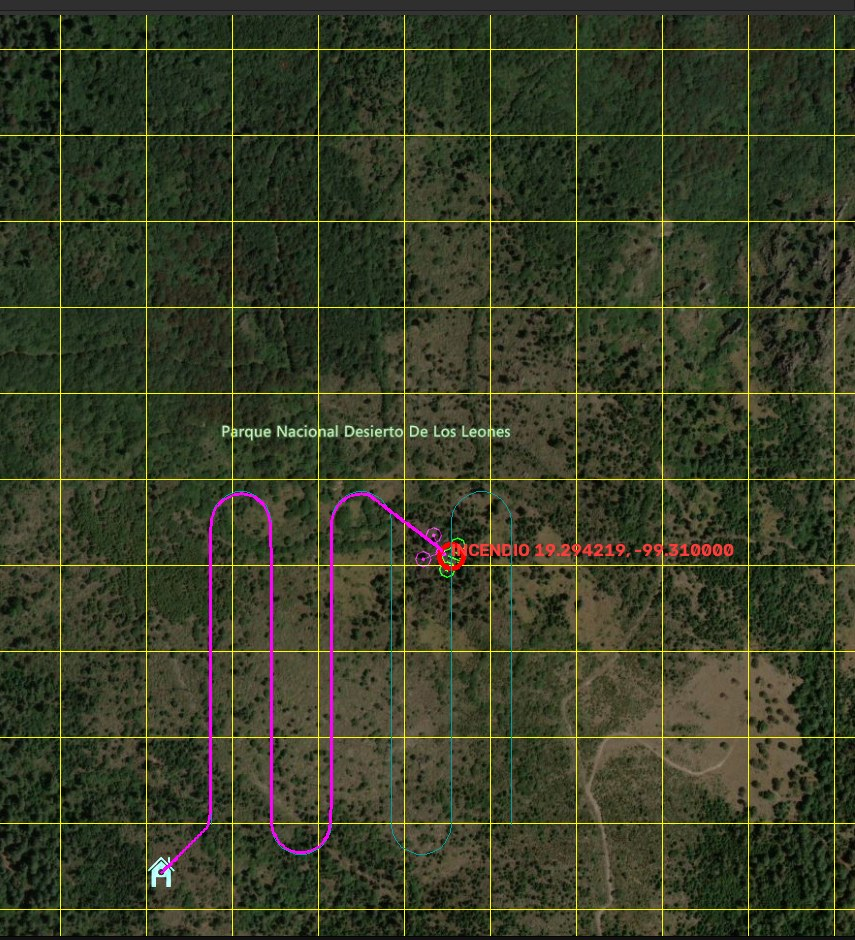
\includegraphics[width=0.6\textwidth]{mapa_trayectoria.jpg}
\caption{Mapa de MAVProxy al final de la búsqueda: trayectoria recorrida desde la base (H), ruta
planeada y foco confirmado.}
\end{figure}

\section{Cierre limpio}

Al cerrar el \emph{launch} con Ctrl-C, un manejador \cod{OnShutdown} termina lo que no se cierra
solo: el \cod{gz sim} que queda detrás del envoltorio de ruby (que no reenvía la señal) y, con
ArduPilot, MAVProxy y ArduCopter, que sim\_vehicle no cierra cuando se cierra su terminal.
